\documentclass[final]{beamer}
\mode<presentation>{\usetheme{PolyU}}
\usepackage[english]{babel}
\usepackage[utf8]{inputenc}
\usepackage[T1]{fontenc}
\usefonttheme{serif}
\usepackage{mathptmx}
\usepackage{amsmath,amssymb}
\usepackage[orientation=portrait,size=a0,scale=1.46]{beamerposter}
\usepackage{graphicx}
\usepackage{booktabs}
\usepackage{array}

\boldmath

\graphicspath{{assets/}}
\setlength{\columnsep}{1.8cm}

\title{BarrierNet: Learning Safe Robot Control\texorpdfstring{\newline}{}with Differentiable CBF}
\author{Yufa You}
\institute[]{Department of Aeronautical and Aviation Engineering, The Hong Kong Polytechnic University}

\begin{document}

\begin{frame}[t]{}
\begin{columns}[t,totalwidth=\textwidth]

\begin{column}{0.31\textwidth}

\begin{block}{Background}
\begin{itemize}
  \item Learned policies perform well but can fail in unseen scenes.
  \item In safety-critical robotics, unsafe actions are unacceptable.
  \item Goal: combine learning flexibility with formal safety guarantees.
  \item BarrierNet treats safety as a trainable module rather than a fixed rule.
\end{itemize}
\end{block}

\begin{block}{Related Work and Gap}
\begin{itemize}
  \item Model-based safe control is often expensive.
  \item Classical CBF filters are safe but hand-tuned and conservative.
  \item Differentiable layers exist, but most do not adapt the safety rule itself.
\end{itemize}

\vspace{0.6cm}
\begin{alertblock}{Research Gap}
\textbf{Need:} an adaptive safety filter that remains formally safe.
\end{alertblock}
\end{block}

\begin{block}{Research Aim}
\begin{itemize}
  \item Plug into a nominal neural controller.
  \item Correct unsafe actions with a differentiable CBF-QP.
  \item Learn safety adaptation from data.
  \item Keep the final action inside a certified safe set.
\end{itemize}
\end{block}

\begin{exampleblock}{Main Takeaway}
% \centering
\Large
Learn the controller \emph{and} the safety adaptation rule together,\\
instead of relying on one fixed barrier design for every situation.
\end{exampleblock}

\begin{block}{Keywords}
% \centering
\large
\textbf{Safe learning}, \textbf{CBF}, \textbf{Differentiable QP}, \textbf{Robot control}
\end{block}

\begin{block}{Poster Summary}
\begin{itemize}
  \item \textbf{Problem:} fixed safety filters are often too conservative.
  \item \textbf{Method:} learn adaptive CBF parameters through a differentiable QP layer.
  \item \textbf{Outcome:} safer control with better task performance.
\end{itemize}
\end{block}

\end{column}

\begin{column}{0.34\textwidth}

\begin{block}{BarrierNet Method}
\begin{center}
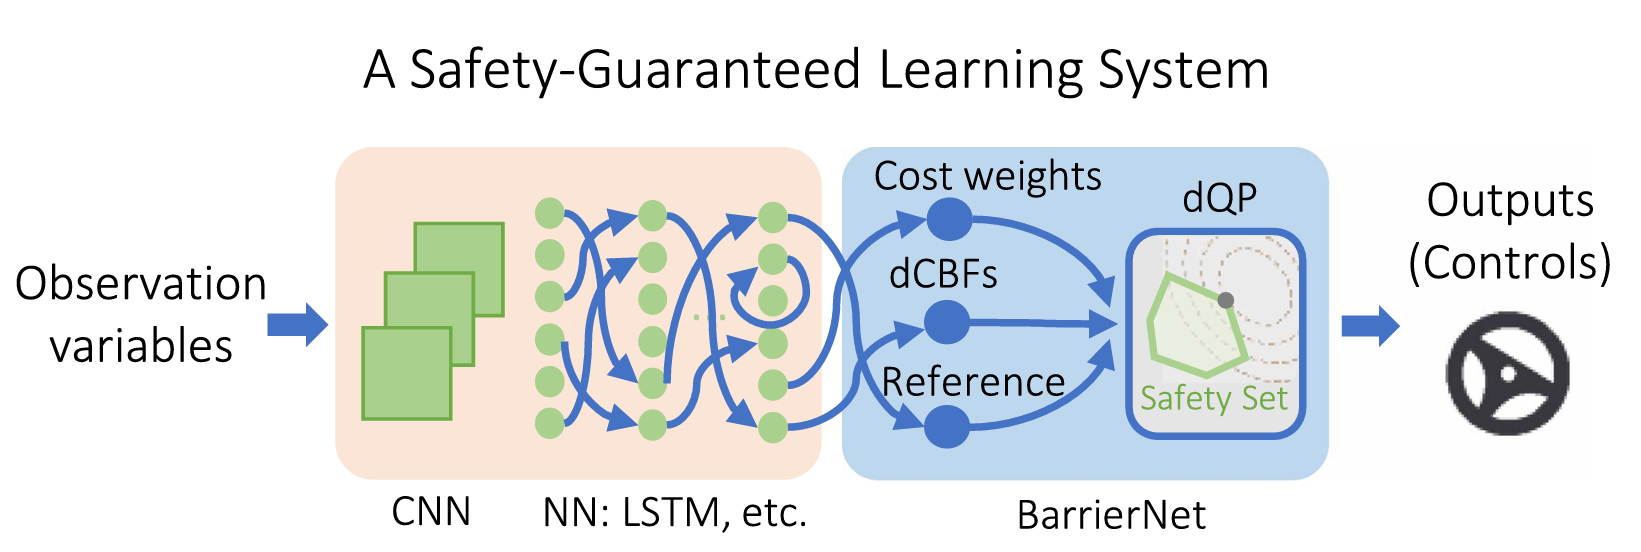
\includegraphics[width=0.96\linewidth]{fig1.png}
\end{center}

\vspace{0.4cm}
\textbf{Pipeline:}
\begin{enumerate}
  \item Nominal policy proposes an action.
  \item BarrierNet predicts adaptive CBF parameters.
  \item A differentiable QP projects to the nearest safe action.
\end{enumerate}
\end{block}

\begin{block}{Core Idea}
For a control-affine system
\[
\dot{x} = f(x) + g(x)u,
\]
BarrierNet enforces a CBF condition of the form
\[
L_f h(x) + L_g h(x)u + \alpha(h(x)) \ge 0,
\]
and computes the safe action by solving
\[
u^\star = \arg\min_u \|u - u_{\text{nom}}\|^2
\]
subject to the safety and actuator constraints.

\vspace{0.5cm}
\textbf{Key idea:} learn the barrier adaptation, not only the policy.
\end{block}

\begin{block}{Why This Matters}
\begin{itemize}
  \item Fewer unnecessary interventions.
  \item Better performance than fixed barriers.
  \item Joint optimization of policy and safety.
\end{itemize}
\end{block}

\begin{exampleblock}{Training Perspective}
\begin{itemize}
  \item The optimization layer is differentiable.
  \item Training encourages policies that are easier to keep safe.
\end{itemize}
\end{exampleblock}

\begin{block}{Compared with Fixed CBF Filters}
\begin{itemize}
  \item Using one setting for all states.
  \item Adapts the safety margin online.
  \item Result: safety-performance balance.
\end{itemize}
\end{block}

\begin{exampleblock}{Take-Home Insight}
% \centering
\large
BarrierNet does not replace CBF theory. It makes the \emph{barrier design}
adaptive enough for learning-based control.
\end{exampleblock}

\begin{exampleblock}{Code}
\centering
\large
https://github.com/Weixy21/BarrierNet

\end{exampleblock}

\end{column}

\begin{column}{0.31\textwidth}

\begin{block}{Experimental Results}
\begin{center}
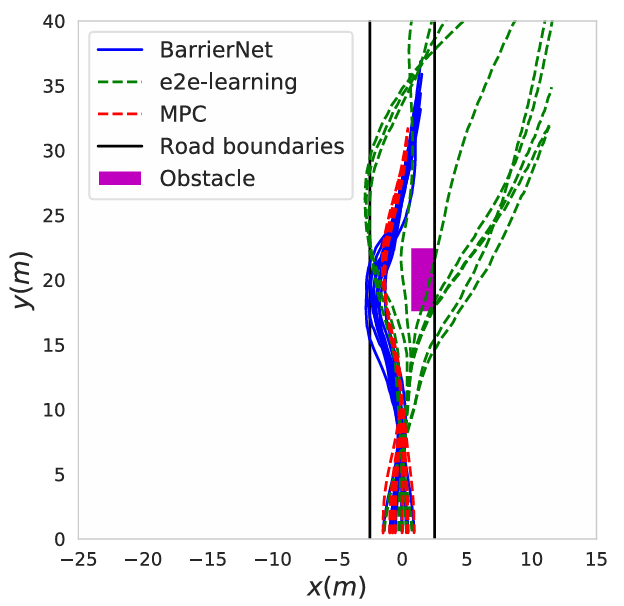
\includegraphics[width=0.97\linewidth]{fig16.png}
\end{center}

\vspace{0.4cm}
\textbf{Observed outcome from the paper:}
\begin{itemize}
  \item Safer than unconstrained learned control.
  \item Less conservative than fixed CBF baselines.
  \item More robust under changing environments and input limits.
\end{itemize}
\end{block}

\begin{block}{Contributions}
\begin{enumerate}
  \item Differentiable CBF safety layer.
  \item Adaptive barrier learning.
  \item Better safety-performance tradeoff.
\end{enumerate}
\end{block}

\begin{exampleblock}{Limitations and Discussion}
\begin{itemize}
  \item Guarantees still depend on model quality.
  \item QP feasibility can remain difficult under tight limits.
\end{itemize}
\end{exampleblock}

\begin{block}{Practical Significance}
\begin{itemize}
  \item Relevant to driving, mobile robots, and manipulators.
  \item Can wrap an existing learned controller.
\end{itemize}
\end{block}

\begin{block}{Reference}
\small
Xiao, W., Cassandras, C. G., and Belta, C. \textit{BarrierNet: Learning Safe Robot Control with Differentiable Control Barrier Functions}. 
\end{block}

\begin{block}{Poster Code}
\small
https://github.com/edyou25/PolyU\_Poster
\end{block}

\end{column}

\end{columns}
\end{frame}

\end{document}
